%\documentclass{standalone}
%\usepackage{graphicx}
%\usepackage[usenames,dvipsnames,svgnames,table]{xcolor}
%\usepackage{tikz}
%\begin{document}
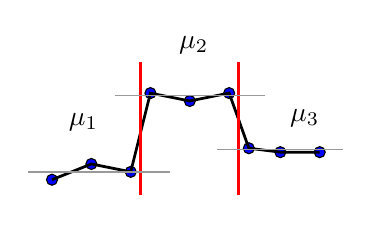
\begin{tikzpicture}[scale = 1]
\def \r {0.07}
    
    \draw[fill=blue] (0.20, 0.90) circle (\r);
    \draw[fill=blue] (0.70, 1.10) circle (\r);
    \draw[fill=blue] (1.20, 1.00) circle (\r);
    
    \draw[fill=blue] (1.45, 2.00) circle (\r);
    \draw[fill=blue] (1.95, 1.90) circle (\r);
    \draw[fill=blue] (2.45, 2.00) circle (\r);
    
    \draw[fill=blue] (2.7, 1.30) circle (\r);
    \draw[fill=blue] (3.10, 1.25) circle (\r);
    \draw[fill=blue] (3.60, 1.25) circle (\r);
    
    \draw[line width=1pt] (0.20, 0.90) -- (0.70, 1.10) -- (1.20, 1.00) -- 
          (1.45, 2.00) -- (1.95, 1.90) -- (2.45, 2.00) -- 
          (2.7, 1.30) -- (3.10, 1.25) -- (3.60, 1.25);
    
    \draw[color=red, line width=1pt] (1.32, 0.70)-- (1.32, 2.4);
    \draw[color=red, line width=1pt] (2.57, 0.70)-- (2.57, 2.4);
    
    % Mean values
    \def \m {1.0} 
    \draw[solid, line width=0.5pt, color = black!40] (-0.1, \m) -- (1.7, \m);
    \node[above] at (-0.1/2 + 1.7/2-0.2, \m+0.4) {$\mu_1$};
    \def \m {1.97} 
    \draw[solid, line width=0.5pt, color = black!40] (1.0, \m) -- (2.9, \m);
    \node[above] at (2, \m + 0.4) {$\mu_2$};
    \def \m {1.28} 
    \draw[solid, line width=0.5pt, color = black!40] (2.3, \m) -- (3.9, \m);
    \node[right] at (2.3/2+3.9/2, \m+0.4) {$\mu_3$};
    
\end{tikzpicture}
%\end{document}
